4. $\cfrac{x(x^2+3)(3-x)(x^3-8)}{(x^2-4)(x+3)^2}\leqslant 0 \Leftrightarrow \cfrac{x(3-x)(x-2)(x^2+2x+4)}{(x-2)(x+2)(x+3)^2}\leqslant 0.$ Применив метод интервалов, найдём ответ: $x\in(-2;0]\cup[3;+\infty).$
\begin{figure}[ht!]
\center{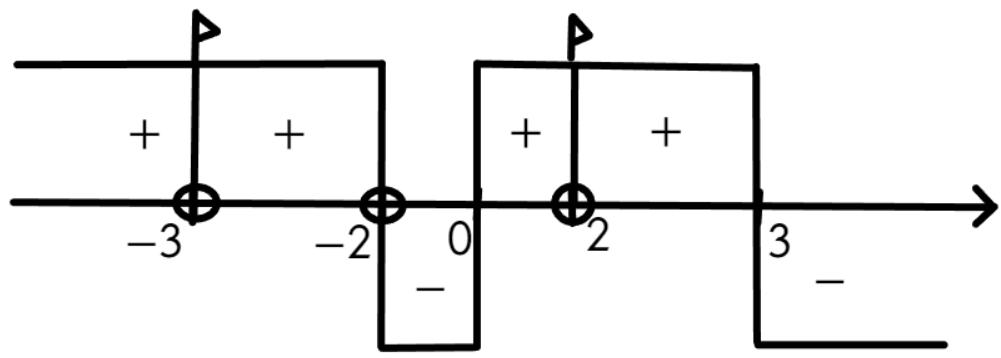
\includegraphics[scale=0.35]{ner9-4.png}}
\end{figure}\\
